%%%%%%%%%%%%%%%%%%%%%%%%%%%%%%%%%%%%%%%%%
% Beamer Presentation
% LaTeX Template
% Version 1.0 (10/11/12)
%
% This template has been downloaded from:
% http://www.LaTeXTemplates.com
%
% License:
% CC BY-NC-SA 3.0 (http://creativecommons.org/licenses/by-nc-sa/3.0/)
%
%%%%%%%%%%%%%%%%%%%%%%%%%%%%%%%%%%%%%%%%%

%----------------------------------------------------------------------------------------
%	PACKAGES AND THEMES
%----------------------------------------------------------------------------------------

\documentclass{beamer}

\mode<presentation> {

% The Beamer class comes with a number of default slide themes
% which change the colors and layouts of slides. Below this is a list
% of all the themes, uncomment each in turn to see what they look like.

%\usetheme{default}
%\usetheme{AnnArbor}
%\usetheme{Antibes}
%\usetheme{Bergen}
%\usetheme{Berkeley}
%\usetheme{Berlin}
%\usetheme{Boadilla}
%\usetheme{CambridgeUS}
%\usetheme{Copenhagen}
%\usetheme{Darmstadt}
%\usetheme{Dresden}
%\usetheme{Frankfurt}
\usetheme{Goettingen}	% vpravo
%\usetheme{Hannover}
%\usetheme{Ilmenau}
%\usetheme{JuanLesPins}
%\usetheme{Luebeck}
%\usetheme{Madrid}
%\usetheme{Malmoe}			
%\usetheme{Marburg}
%\usetheme{Montpellier}
%\usetheme{PaloAlto}
%\usetheme{Pittsburgh}
%\usetheme{Rochester}
%\usetheme{Singapore}			
%\usetheme{Szeged}
%\usetheme{Warsaw}

% As well as themes, the Beamer class has a number of color themes
% for any slide theme. Uncomment each of these in turn to see how it
% changes the colors of your current slide theme.

%\usecolortheme{albatross}
%\usecolortheme{beaver}
%\usecolortheme{beetle}
%\usecolortheme{crane}
%\usecolortheme{dolphin}
%\usecolortheme{dove}
%\usecolortheme{fly}
%\usecolortheme{lily}			
%\usecolortheme{orchid}
%\usecolortheme{rose}
%\usecolortheme{seagull}
%\usecolortheme{seahorse}
%\usecolortheme{whale}
%\usecolortheme{wolverine}

%\setbeamertemplate{footline} % To remove the footer line in all slides uncomment this line
%\setbeamertemplate{footline}[page number] % To replace the footer line in all slides with a simple slide count uncomment this line

%\setbeamertemplate{navigation symbols}{} % To remove the navigation symbols from the bottom of all slides uncomment this line
}

\usepackage[utf8]{inputenc}	% kódování textu
\usepackage[english]{babel}		% zavedení češtiny
\usepackage{amsmath,amsfonts,amssymb}	% matematika
\usepackage{graphicx} % Allows including images
\usepackage{booktabs} % Allows the use of \toprule, \midrule and \bottomrule in tables
\usepackage{multirow}	% slouceni radek v tabulce
\usepackage{multicol}	% slouceni sloupcu v tabulce
\usepackage{longtable}	% rozdeleni tabulky pres vice stran
\usepackage{enumerate}	% seznamy
\usepackage{float}
\usepackage{lscape}		% stranka na sirku
\usepackage{fancyhdr}
\usepackage{url}
\usepackage{array}
\usepackage{subfigure}
\usepackage{dirtree}
\usepackage{setspace}
\usepackage{color}
\usepackage{listings}
\usepackage{multimedia}
\usepackage{tikz}
\usepackage{fancyvrb}


%------------------------------------------------------------------
%	TITLE PAGE
%------------------------------------------------------------------

\title[]{GPU usage at JEODPP platform} % The short title appears at the bottom of every slide, the full title is only on the title page

\iffalse
\author{Ondřej Pešek} % Your name
\institute[ČVUT] % Your institution as it will appear on the bottom of every slide, may be shorthand to save space
{
České vysoké učení technické v Praze \\ % Your institution for the title page
%\medskip
Fakulta stavební \\
%\medskip
Obor Geomatika
}
\date{20. 6. 2018} % Date, can be changed to a custom date
\titlegraphic{
\includegraphics[width=1.5cm]{pictures/logo2.pdf}}
\fi

\begin{document}

\begin{frame}
\titlepage % Print the title page as the first slide
\end{frame}

\begin{frame}
\frametitle{Table of contents} % Table of contents slide, comment this block out to remove it
\tableofcontents % Throughout your presentation, if you choose to use \section{} and \subsection{} commands, these will automatically be printed on this slide as an overview of your presentation
\end{frame}

%------------------------------------------------------------------
%	PRESENTATION SLIDES
%------------------------------------------------------------------
\iffalse
%------------------------------------------------------------------
\section{Motivace} % Sections can be created in order to organize your presentation into discrete blocks, all sections and subsections are automatically printed in the table of contents as an overview of the talk
%------------------------------------------------------------------

\begin{frame}

\frametitle{Motivace}

Situace
\begin{itemize}
	\item posilování satelitní sítě
	\item posilování leteckého snímkování
	\item vektorizace skenovaných map
	\visible<2->{\item zlepšování kvality snímků}
	\visible<3->{\item otevírání dat}
	\visible<4->{\item standardizace dat}
\end{itemize}

\end{frame}

%------------------------------------------------------------------

\begin{frame}

\frametitle{Motivace}

Běžné způsoby klasifikace
\begin{itemize}
	\item ruční klasifikace
	\visible<2->{\item řízená klasifikace}
	\visible<3->{\item neřízená klasifikace}
\end{itemize}

\bigskip

GRASS GIS
\begin{itemize}
	\item ruční klasifikace
	\begin{itemize}
		\item GRASS Digitizing tool
	\end{itemize}
	\visible<2->{\item řízená klasifikace
	\begin{itemize}
		\item g.gui.iclass + i.maxlik
	\end{itemize}}
	\visible<3->{\item neřízená klasifikace
	\begin{itemize}
		\item i.cluster + i.maxlik
	\end{itemize}}
\end{itemize}

\end{frame}

%------------------------------------------------------------------

\begin{frame}

\frametitle{Motivace}

Proč neuronové sítě?
\begin{itemize}
	\item mozek je nejsilnější nástroj, který máme dispozici
	\item snažíme se dosáhnout lidsky srozumitelných výsledků
\end{itemize}

\begin{figure}[ht]
	\includegraphics<1>[width=0.55\textwidth]{pictures/nn1.png}
	\includegraphics<2>[width=0.65\textwidth]{pictures/nn2.png}
	\includegraphics<3>[width=0.55\textwidth]{pictures/nn3.jpg}
	\caption{Zdroj: [1]}
\end{figure}

\end{frame}
\fi
%------------------------------------------------------------------

\section{Theoretical framework}
\iffalse
\subsection{Convolutional neural networks} % A subsection can be created just before a set of slides with a common theme to further break down your presentation into chunks

%------------------------------------------------------------------

\begin{frame}

\frametitle{Convolutional neural networks}

\begin{figure}[ht]
	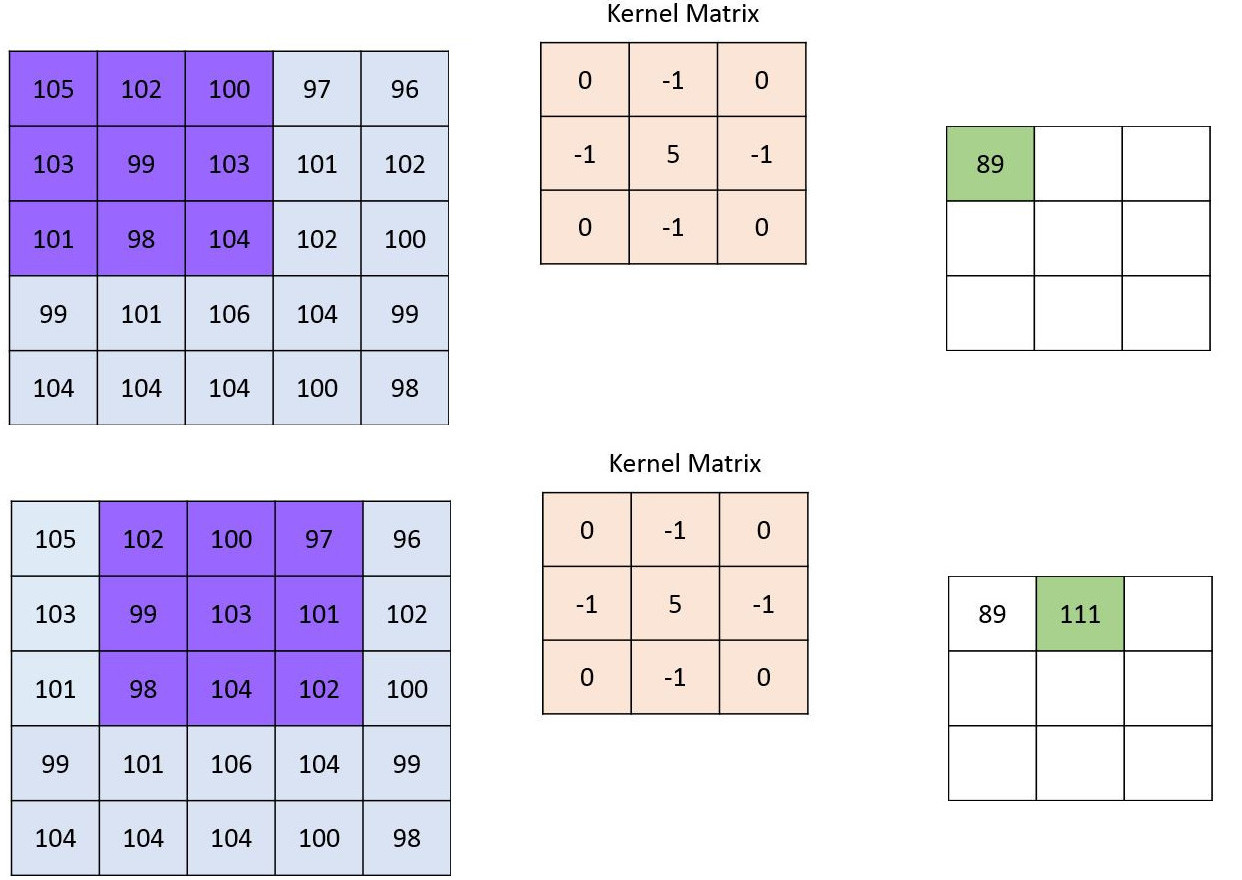
\includegraphics[width=0.6\textwidth]{pictures/conv.jpg}
\end{figure}

\visible<2->{Why convolutional neural networks?
\begin{itemize}
	\item ResNet got in ILSVRC 2016 top 5 error of 3.6 \%
	\item<3> human 8 \%
\end{itemize}

Source: [1]}

\end{frame}
\fi
%------------------------------------------------------------------

\subsection{Instance segmentation}

\begin{frame}

\frametitle{Instance segmentation}

%\visible<2>{Instance segmentation}

\begin{figure}[ht]
	\includegraphics<1>[width=0.9\textwidth]{pictures/segmentations.png}
	%\includegraphics<2>[width=0.65\textwidth]{pictures/instance-segmentation.png}
	\caption{Source: [1]}
\end{figure}

\end{frame}

%------------------------------------------------------------------

\subsection{Mask R-CNN}

\begin{frame}

\frametitle{Mask R-CNN}

Two parts:
\begin{itemize}
	\item backbone
	\item head
\end{itemize}

\begin{figure}[ht]
	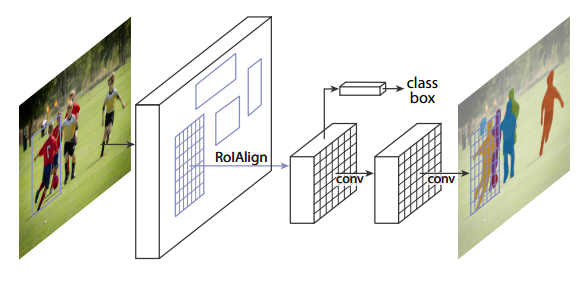
\includegraphics[width=0.8\textwidth]{pictures/maskrcnn.png}
	\caption{Source: [2]}
\end{figure}

\end{frame}

%------------------------------------------------------------------

\iffalse

\begin{frame}

\frametitle{Mask R-CNN}

Backbone architecture:
\begin{itemize}
	\item ResNet
	\item<2-> RPN
\end{itemize}

\begin{figure}[ht]
	\includegraphics<1>[width=0.5\textwidth]{pictures/bottleneck-block.jpg}
	\includegraphics<2>[width=0.5\textwidth]{pictures/fasterrcnn.png}
	\includegraphics<3>[width=0.5\textwidth]{pictures/fasterrcnn-anchors.png}
	\caption{Source: [3]}
\end{figure}

\end{frame}

%------------------------------------------------------------------

\begin{frame}

\frametitle{Mask R-CNN}

Head architecture:
\begin{itemize}
	\item softmax $\rightarrow$ class
	\item<2-> regression $\rightarrow$ bounding box
	\item<3-> FCN $\rightarrow$ mask
\end{itemize}

\begin{figure}[ht]
	\includegraphics<1-2>[width=\textwidth]{pictures/fastrcnn.png}
	\includegraphics<3>[width=\textwidth]{pictures/maskrcnn-head.png}
	\caption{Source: [4]}
\end{figure}

\end{frame}

\fi

%------------------------------------------------------------------

\section{Tools}

%------------------------------------------------------------------

\subsection{Usage}

\begin{frame}

\frametitle{Usage}

Software:

\begin{center}
\includegraphics[scale=1]{../text/pictures/grass-logo.png}
\end{center}

Workflow:
\begin{itemize}
	\item i.ann.maskrcnn.train
	\item i.ann.maskrcnn.detect
\end{itemize}

\end{frame}

%------------------------------------------------------------------

\subsection{i.ann.maskrcnn.train}

\begin{frame}

\frametitle{i.ann.maskrcnn.train}

\begin{figure}[ht]
	\includegraphics<1>[width=.7\textwidth]{pictures/Screenshotfrom2018-09-2610-31-45.png}
	\includegraphics<2>[width=.7\textwidth]{pictures/Screenshotfrom2018-09-2610-3428.png}
\end{figure}

\end{frame}

%------------------------------------------------------------------

\subsection{i.ann.maskrcnn.detect}

\begin{frame}

\frametitle{i.ann.maskrcnn.detect}

\begin{figure}[ht]
	\includegraphics<1>[width=.7\textwidth]{pictures/Screenshotfrom2018-09-2610-3222.png}
	\includegraphics<2>[width=.7\textwidth]{pictures/Screenshotfrom2018-09-2610-3520.png}
\end{figure}

\end{frame}

%------------------------------------------------------------------

\subsection{Outputs}

\begin{frame}

\frametitle{Outputs}

\begin{figure}[ht]
	%\only<1>{
	%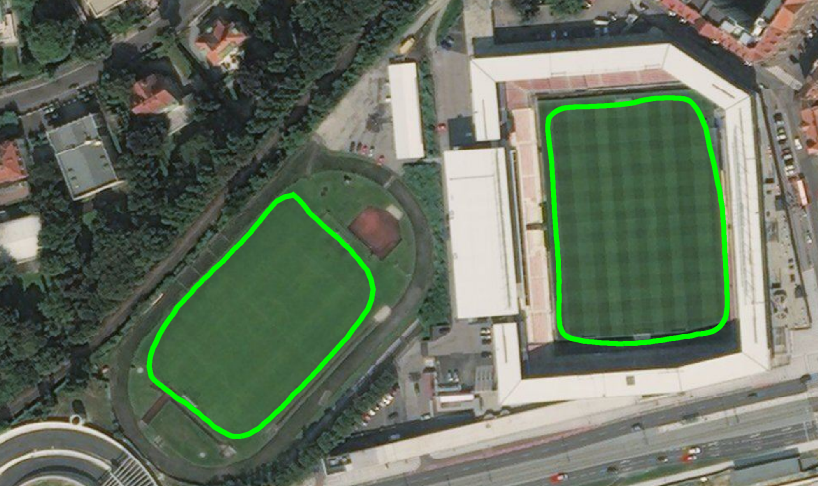
\includegraphics[width=.9\textwidth]{pictures/out1.png}
	%\caption{loss function 0.96, 54000 training images}}
	\only<1>{
	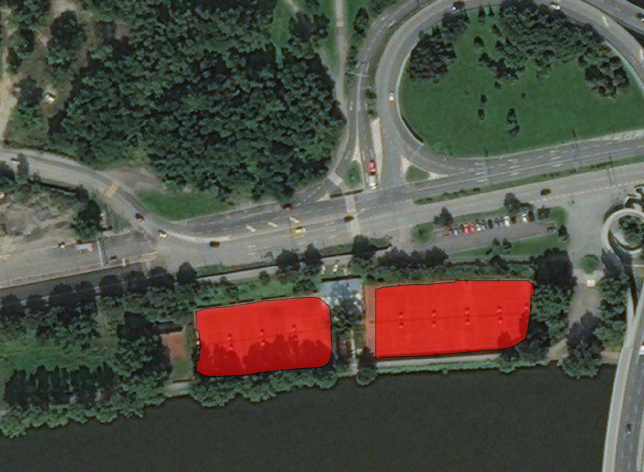
\includegraphics[width=.9\textwidth]{pictures/out2.png}
	\caption{loss function 0.96, 54000 training images}}
	\only<2>{
	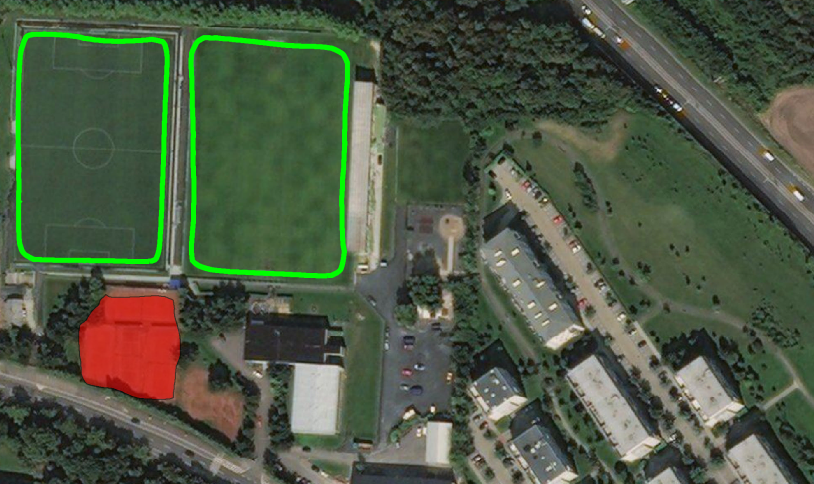
\includegraphics[width=.9\textwidth]{pictures/out3.png}
	\caption{loss function 0.96, 54000 training images}}
	%\only<4>{
	%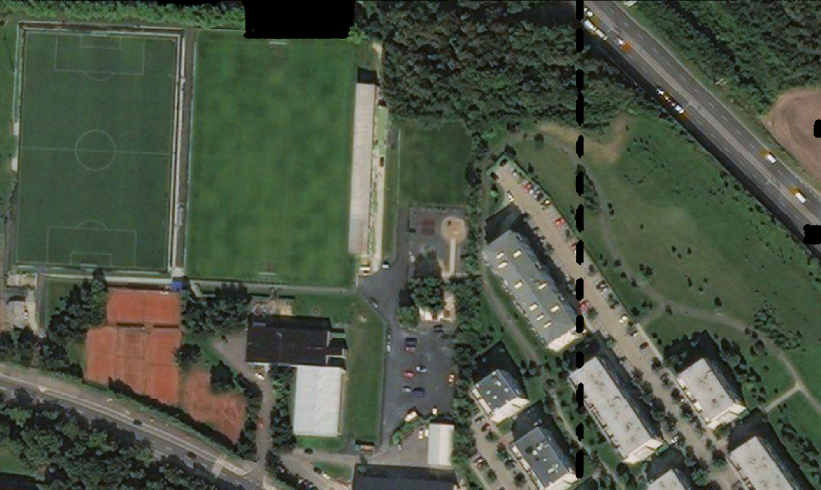
\includegraphics[width=.9\textwidth]{pictures/out_b_1.png}
	%\caption{epoch 1, loss function 35.01, 2400 training images}}
	%\only<5>{
	%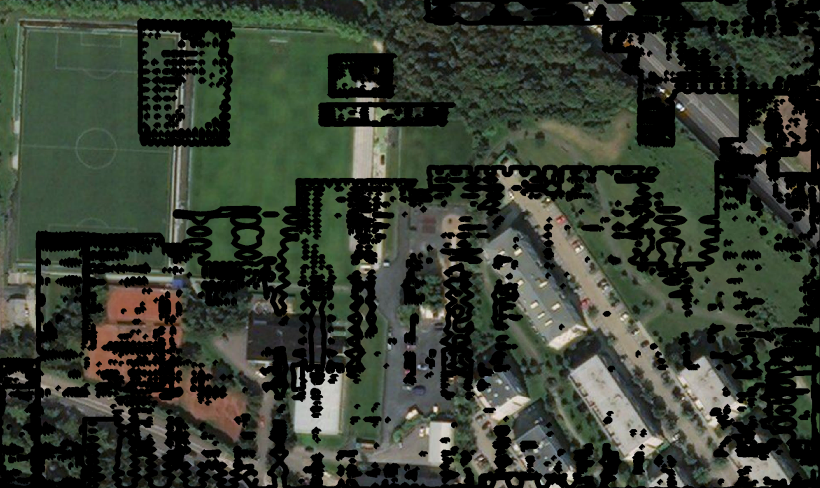
\includegraphics[width=.9\textwidth]{pictures/out_b_10.png}
	%\caption{epoch 10, loss function 5.87, 2400 training images}}
	%\only<6>{
	%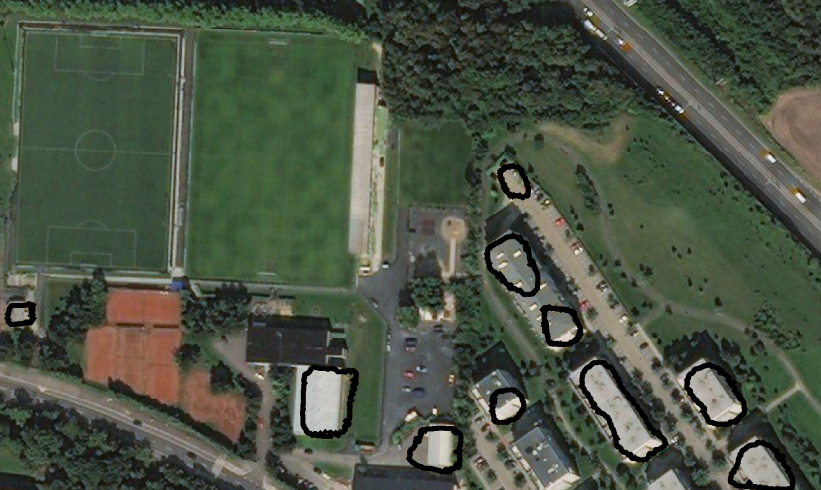
\includegraphics[width=.9\textwidth]{pictures/out_b_50.png}
	%\caption{epoch 50, loss function 1.36, 2400 training images}}
	\only<3>{
	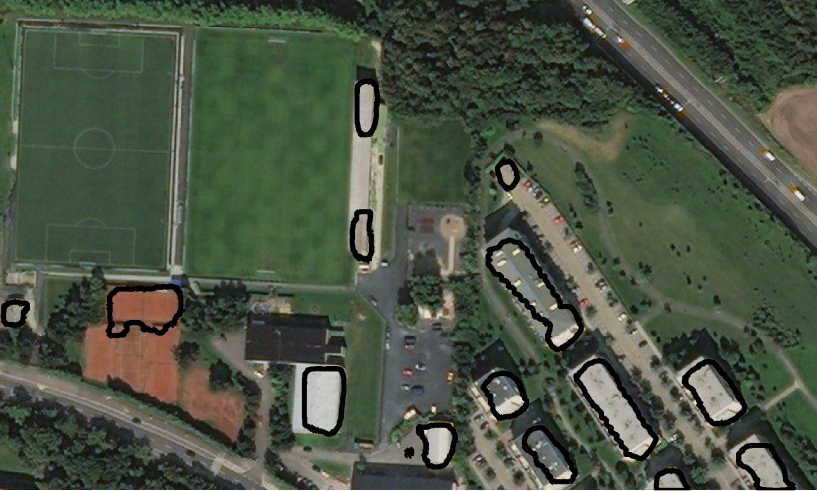
\includegraphics[width=.9\textwidth]{pictures/out_b_150.png}
	\caption{epoch 150, loss function 0.63, 2400 training images}}
	%\only<8>{
	%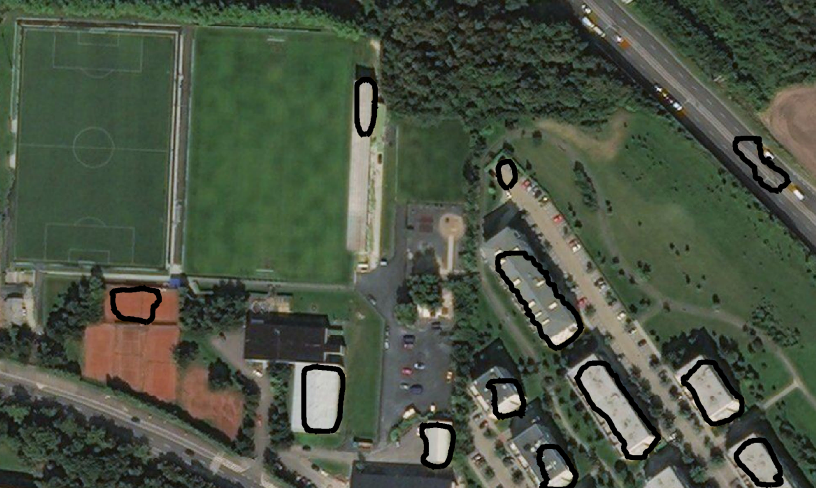
\includegraphics[width=.9\textwidth]{pictures/out_b_180.png}
	%\caption{epoch 180, loss function 0.50, 2400 training images}}
\end{figure}

\end{frame}

%------------------------------------------------------------------

\section{Tools availability}

\begin{frame}[fragile]

\frametitle{Tools availability}

\begin{itemize}
	\item source code
	\begin{itemize}
		%\item \url{https://github.com/ctu-geoforall-lab-projects/dp-pesek-2018}
		\item \url{https://github.com/ctu-geoforall-lab/i.ann.maskrcnn}
		\item \url{https://svn.osgeo.org/grass/grass-addons/grass7/imagery/i.ann.maskrcnn/}
	\end{itemize}
	\item installation using command \verb|g.extension extension=i.ann.maskrcnn|
	%\item next steps
	%\begin{itemize}
	%	\item multispectral rasters
	%	\item training on rasters and vectors imported in GRASS
	%	\item more architectures
	%\end{itemize}
\end{itemize}

\end{frame}

%------------------------------------------------------------------

\section{Statistics}

\begin{frame}

\frametitle{Statistics}

\fontsize{5}{6}\selectfont{
\setlength\tabcolsep{2.4pt}
\begin{tabular}{l*{6}{c}}
Processing units & Seconds per image & GPU usage [\%] & GPU memory usage [MB] & CPU relative load & Main memory usage [GB] \\
\hline
20 CPUs & 9.937 & 0 & 0 & 0.18 & 147.7    \\
1 GPU & 3.945 & 81 & 11.31 & 0.06 & 151.1  \\
2 GPUs & 3.711 & 69 & 11.31 & 0.06 & 115.8  \\
3 GPUs & 3.456 & 58 & 11.31 & 0.07 & 173.7   \\
4 GPUs & 3.010 & 46 & 11.31 & 0.08 & 219.9   \\
\end{tabular}
}

\vspace{15px}

\visible<2->{
\fontsize{5}{6}\selectfont{
\setlength\tabcolsep{2.4pt}
\begin{tabular}{l*{2}{c}}
Processing units & Images per GPU & Seconds per image \\
\hline
1 GPU & 4 & 4.250 \\
4 GPUs & 1 & 3.010  \\
\end{tabular}
}
}

\vspace{15px}

\visible<3->{
\fontsize{5}{6}\selectfont{
\setlength\tabcolsep{2.4pt}
\begin{tabular}{l*{2}{c}}
Processing units & Number of simultaneous processes & Seconds per image \\
\hline
1 GPU & 1 & 3.945 \\
1 GPU & 2 & 3.999  \\
\\
2 GPUs & 1 & 3.711 \\
2 GPUs & 2 & 3.762  \\
\end{tabular}
}
}


\end{frame}

%------------------------------------------------------------------

\section{Conclusion}

\begin{frame}

\frametitle{Conclusion}

\begin{itemize}
\item 1 GPU is in average 2.5 times faster than 20 CPUs
\item<2-> 4 GPUs are in average 1.5 times faster than 1 GPU
\item<3-> GPUs with 1 image loaded per GPU are in average 1.5 faster than 1 GPU with 4 images per GPU
\item<4-> GPU with restricted access to the memory of other GPUs reaches almost the same speed as with access
\item<5-> The optimal solution is to allow multiuser usage with access to 1 GPU per docker
\end{itemize}

\end{frame}

%------------------------------------------------------------------

\section{Sources}

\begin{frame}

\frametitle{Sources}

[1] http://cs231n.stanford.edu/

[2] HE, Kaiming et al. Mask R-CNN. In: International Conference on Computer
Vision (ICCV). 2017.

\end{frame}

%------------------------------------------------------------------

\begin{frame}

\centerline{Thank you for your attention.}

\end{frame}

%------------------------------------------------------------------
\iffalse
\section{Reakce na otázky oponenta}

\begin{frame}

\frametitle{Reakce na otázky oponenta}

Jaké jsou výhody/nevýhody užití neuronových sítí namísto klasických postupů?

\begin{center}
	\noindent\makebox[\linewidth]{\rule{0.9\textwidth}{0.4pt}}
\end{center}

\bigskip

Výhody:
\begin{itemize}
	\item<2-> přesnost
	\item<3-> minimalizovaná potřeba vytvářet ad hoc řešení
	\item<4-> obecnost
\end{itemize}

Nevýhody:
\begin{itemize}
	\item<5-> výpočetní náročnost
	\item<6-> časová náročnost
	\item<7-> potřeba rozsáhlých trénovacích dat
	\item<8-> odvážným štěstí nepřeje vždy
\end{itemize}

\end{frame}

%------------------------------------------------------------------

\begin{frame}

\frametitle{Reakce na otázky oponenta}

Implementoval jste modifikace využitého software i zpět do zdrojů?

\begin{center}
	\noindent\makebox[\linewidth]{\rule{0.9\textwidth}{0.4pt}}
\end{center}

\bigskip

Ano:
\begin{itemize}
	\item<2-> GRASS GIS
\end{itemize}

Ne:
\begin{itemize}
	\item<3-> GRASS GIS
	\item<4-> Matterport, Inc.
	\item<7-> potřeba rozsáhlých trénovacích dat
	\item<8-> odvážným štěstí nepřeje vždy
\end{itemize}

\end{frame}

%------------------------------------------------------------------

\begin{frame}

\frametitle{Reakce na otázky oponenta}

Shledáváte některé části svého kódu natolik obecnými, aby mohly být využiti i při vývoji dalších podobných nástrojů?

\begin{center}
	\noindent\makebox[\linewidth]{\rule{0.9\textwidth}{0.4pt}}
\end{center}

\bigskip

\visible<2->{Ano.}

\end{frame}

%------------------------------------------------------------------

\begin{frame}

\frametitle{Reakce na otázky oponenta}

V textu práce jste zmínil a rozebíral podezřelé chování modulů skýtajících lepší výsledky při vyšší ztrátové funkci. Můžete tento případ ještě rozvést?

\begin{center}
	\noindent\makebox[\linewidth]{\rule{0.9\textwidth}{0.4pt}}
\end{center}

\bigskip

Možné příčiny:
\begin{itemize}
	\item<2-> přeoptimalizace
	\item<3-> lokální odchylka
	\item<4-> nedostatečná data
\end{itemize}

\begin{figure}
	\centering
	\begin{minipage}{.45\textwidth}
		\centering
		\begin{figure}[ht]
	  		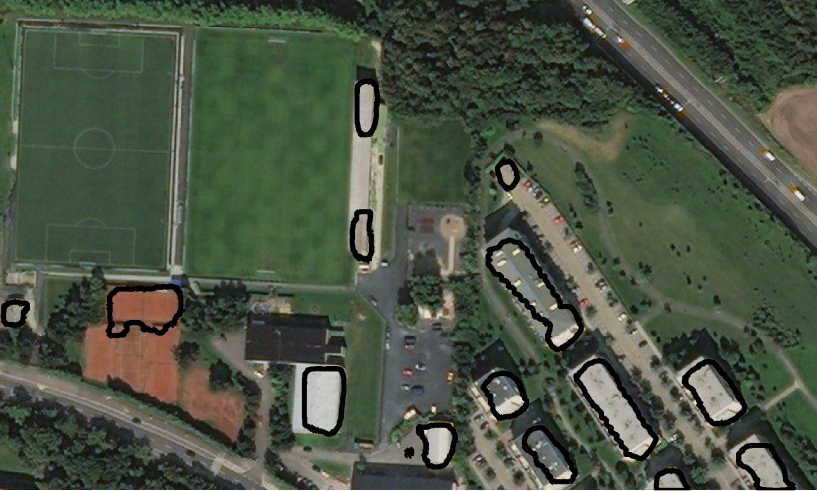
\includegraphics[width=4.5cm]{pictures/out_b_150.png}
		\end{figure}
    \end{minipage}%
    \begin{minipage}{.6\textwidth}
		\centering
		\begin{figure}[ht]
			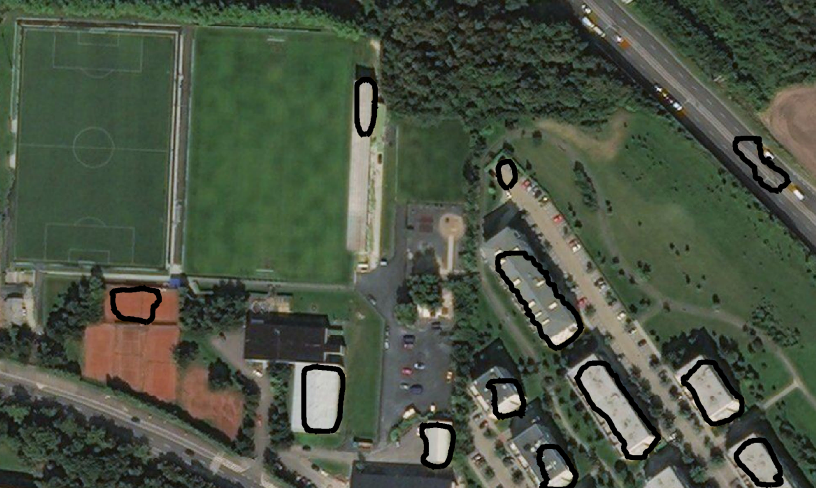
\includegraphics[width=4.5cm]{pictures/out_b_180.png}
		\end{figure}
	\end{minipage}
\end{figure}

\end{frame}
\fi
%==================================================================
\end{document} 

